% This file is part of xrayutilities.
%
% xrayutilities is free software; you can redistribute it and/or modify 
% it under the terms of the GNU General Public License as published by 
% the Free Software Foundation; either version 2 of the License, or 
% (at your option) any later version.
%
% This program is distributed in the hope that it will be useful,
% but WITHOUT ANY WARRANTY; without even the implied warranty of
% MERCHANTABILITY or FITNESS FOR A PARTICULAR PURPOSE.  See the
% GNU General Public License for more details.
%
% You should have received a copy of the GNU General Public License
% along with this program; if not, see <http://www.gnu.org/licenses/>.
%
% Copyright (C) 2009 Eugen Wintersberger <eugen.wintersberger@desy.de>
% Copyright (C) 2010 Dominik Kriegner <dominik.kriegner@aol.at>

\documentclass[a4paper]{book}
\usepackage{amsmath,graphics,listings,hyperref,pdfpages,placeins,float}
\hypersetup{pdftitle=XRUTILS manual,
				pdfborder=0 0 0,
				colorlinks=false}
\lstset{ %
language=Python,                % choose the language of the code
basicstyle=\footnotesize,       % the size of the fonts that are used for the code
showspaces=false,               % show spaces adding particular underscores
showstringspaces=false,         % underline spaces within strings
showtabs=false,                 % show tabs within strings adding particular underscores
frame=single,	                % adds a frame around the code
captionpos=b,                   % sets the caption-position to bottom
breaklines=true,                % sets automatic line breaking
breakatwhitespace=true,        % sets if automatic breaks should only happen at whitespace
title=\lstname,                 % show the filename of files included with \lstinputlisting; also try caption instead of title
escapeinside={\#*}{*)}          % if you want to add a listings comment #* comment *
}

%%%%%%%%%%%%%%%%%%%%%%%%%%%%%%
%%%%   maths packages   %%%%%%
%%%%%%%%%%%%%%%%%%%%%%%%%%%%%%
\usepackage{amsmath}
\usepackage{amssymb,amstext}
\usepackage{ulem}
\usepackage{textcomp} %% Mathe/Textsymbole
\usepackage{stmaryrd}
\usepackage{units}
\usepackage[thinspace,mediumqspace,Gray,squaren]{SIunits}

\renewcommand{\vec}[1]{
	\ensuremath{\boldsymbol{#1}}
}
\newcommand{\mat}[1]{\ensuremath{\uuline{#1}}}
\newcommand{\av}[1]{\ensuremath{\left< #1 \right>}}
\newcommand{\pprime}{\ensuremath{ {\prime\prime}  }}


\newenvironment{nomenclatur}
{
\begin{list}{}
{
\renewcommand{\makelabel}[1]{\ensuremath{##1} \dotfill} 
\setlength{\labelwidth}{2.7cm}  
\setlength{\labelsep}{0.25cm}
\setlength{\topsep}{0.5ex}
\setlength{\itemsep}{-1.1ex}  
\setlength{\leftmargin}{2.95cm} %\labelwidth+\labelsep
}}
{\end{list}}


\title{{\Huge XRUTILS Users Manual}}
\author{Eugen Wintersberger \and with contributions from Dominik Kriegner}

\begin{document}
\maketitle
\tableofcontents

\chapter{Introduction}
% This file is part of xrayutilities.
%
% xrayutilities is free software; you can redistribute it and/or modify 
% it under the terms of the GNU General Public License as published by 
% the Free Software Foundation; either version 2 of the License, or 
% (at your option) any later version.
%
% This program is distributed in the hope that it will be useful,
% but WITHOUT ANY WARRANTY; without even the implied warranty of
% MERCHANTABILITY or FITNESS FOR A PARTICULAR PURPOSE.  See the
% GNU General Public License for more details.
%
% You should have received a copy of the GNU General Public License
% along with this program; if not, see <http://www.gnu.org/licenses/>.
%
% Copyright (C) 2010 Dominik Kriegner <dominik.kriegner@aol.at>

%%% Introduction

pass :-)
 
%%% About the documentation 

\section{About this document}

The purpose of this file is mainly to provide a starting point for new users and a repository of usage examples for xrutils. Feel free to add new things, change errors and expand the examples as you think it is useful.


\chapter{Installation}
%%%installation notes

Installing {\tt xrutils} is a three steps process
\begin{enumerate}
\item install required C libraries and Python modules
\item build and install the {\tt xrutils} C library
\item install the Python module
\end{enumerate}
All steps are described in detail in this chapter.

\section{Required third party software}
To keep the coding effort as small as possible {\tt xrutils} depends on a 
large number of third party libraries and Python modules. 

The following C/C++ libraries are needed 
\begin{description}
\item[VTK] the Visualization Toolkit, a large C++ library for 3D data
visualization
\item[HDF5] a versatile binary data format (library is implemented in C).
Although the library is not called directly, it is needed by the pytables Python
module (see below).
\end{description}

Additionally, the following Python modules must be installed in order to make 
{\tt xrutils} work as intended
\begin{description}
\item[Numpy] a Python module providing numerical array objects
\item[VTK Python bindings] usually contained in the VTK distribution, however,
on some system the Python bindings must be installed separately 
\item[Python-Tables] a powerful Python interface to HDF5
\item[Matplotlib] a Python module for high quality 1D and 2D plotting
\item[pyvtk] reading and writing legacy VTK files
\end{description}
After installing all required packages you can continue with installing and
building the C library.

\section{Building and installing the C library}

{\tt xrutils} user the SCons build system to compile the C components of the
system. You can build the library simply by typing 
\begin{verbatim}
>scons
\end{verbatim}
in the root directory of the source distribution. After building the library can
be installed with
\begin{verbatim}
>scons install --prefix=<install path>
\end{verbatim}
The library is installed in {\tt<install path>/lib}. It is absolutely necessary
to perform this step before installing the Python module since during
installation of the C library a file {\tt config.py} is created in the top
package of the Python module containing the path to the C library. This is in so
far important that the {\tt ctypes} module used to access C library functions
uses this path to find the library. In principal this step could have been
omitted on Linux systems where environment variables can be used to tell the
system where to look for shared libraries. However, on Windows systems, for
instance, no such facility exists and therefore, relying on such mechanisms
would make the installation process highly platform dependent. 

The documentation can be build with 
\begin{verbatim}
>scons doc
\end{verbatim}
which creates this file under {\tt doc/manual/}.

Finally after installing the C library you can continue with installing the
Python module.

\section{Installing the Python package}

Installation of the Python module is done via the {\tt distutils} package
shipped with every Python distribution. Actually, two installation modes are 
supported
\begin{itemize}
 \item system wide installation in the system wide Python installation
 \item local to a single user only.
\end{itemize}

In the first case, to install {\tt xrutils} into the global Python installation
simply run
\begin{verbatim}
>python setup.py
\end{verbatim}
From the root directory of the {\tt xrutils} source distribution (this is the
directory where also the {\tt SConstruct} file resides). Since your system-wide
Python installation is setup correctly you are done with the installation.

If you want to install
{\tt xrutils} only local to a single user use
\begin{verbatim}
>python setup.py --home=<local install path>
\end{verbatim}
In this case the {\tt xrutils} package is installed under {\tt <local install
path>/lib/python}. Finally you need to make your Python installation aware of
were to look for the module. For this case append the installation directory to
your {\tt PYTHONPATH} environment variable by 
\begin{verbatim}
>export PYTHONPATH=$PYTHONPATH:<local install path>/lib/python
\end{verbatim}
on a terminal. Or, to make this configuration persistent append this line to
your local {\tt .bashrc} file in your home directory.


\chapter{Basic concepts}
% This file is part of xrayutilities.
%
% xrutils is free software; you can redistribute it and/or modify 
% it under the terms of the GNU General Public License as published by 
% the Free Software Foundation; either version 2 of the License, or 
% (at your option) any later version.
%
% This program is distributed in the hope that it will be useful,
% but WITHOUT ANY WARRANTY; without even the implied warranty of
% MERCHANTABILITY or FITNESS FOR A PARTICULAR PURPOSE.  See the
% GNU General Public License for more details.
%
% You should have received a copy of the GNU General Public License
% along with this program; if not, see <http://www.gnu.org/licenses/>.
%
% Copyright (C) 2009 Eugen Wintersberger <eugen.wintersberger@desy.de>
% Copyright (C) 2010 Dominik Kriegner <dominik.kriegner@aol.at>

%%% basic usage principles of xrutils

This chapter describes two concepts of usage for the {\tt xrutils} package, which help with planning and analyzing experiments.

First the flowchart of how angular coordinates of Bragg reflections are calculated is shown (Fig.~\ref{fig:xrutils_usage_planning}). After that a sketch on how to analyze x-ray diffraction data with {\tt xrutils} is shown in Fig.~\ref{fig:xrutils_usage}. More detailed descriptions of the steps described here given in the subsequent chapters.

\begin{figure}[H]
 \centering
 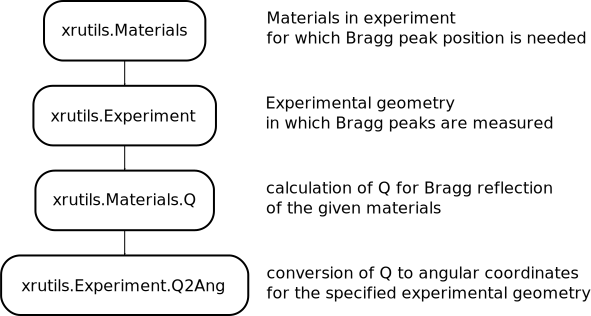
\includegraphics[width=0.8\linewidth]{pics/xrutils_usage_planning}
 \caption{Flow diagram showing how to calculate angular positions of Bragg reflection using {\tt xrutils}.}
 \label{fig:xrutils_usage_planning}
\end{figure}
   
\begin{figure}[H]
 \centering
 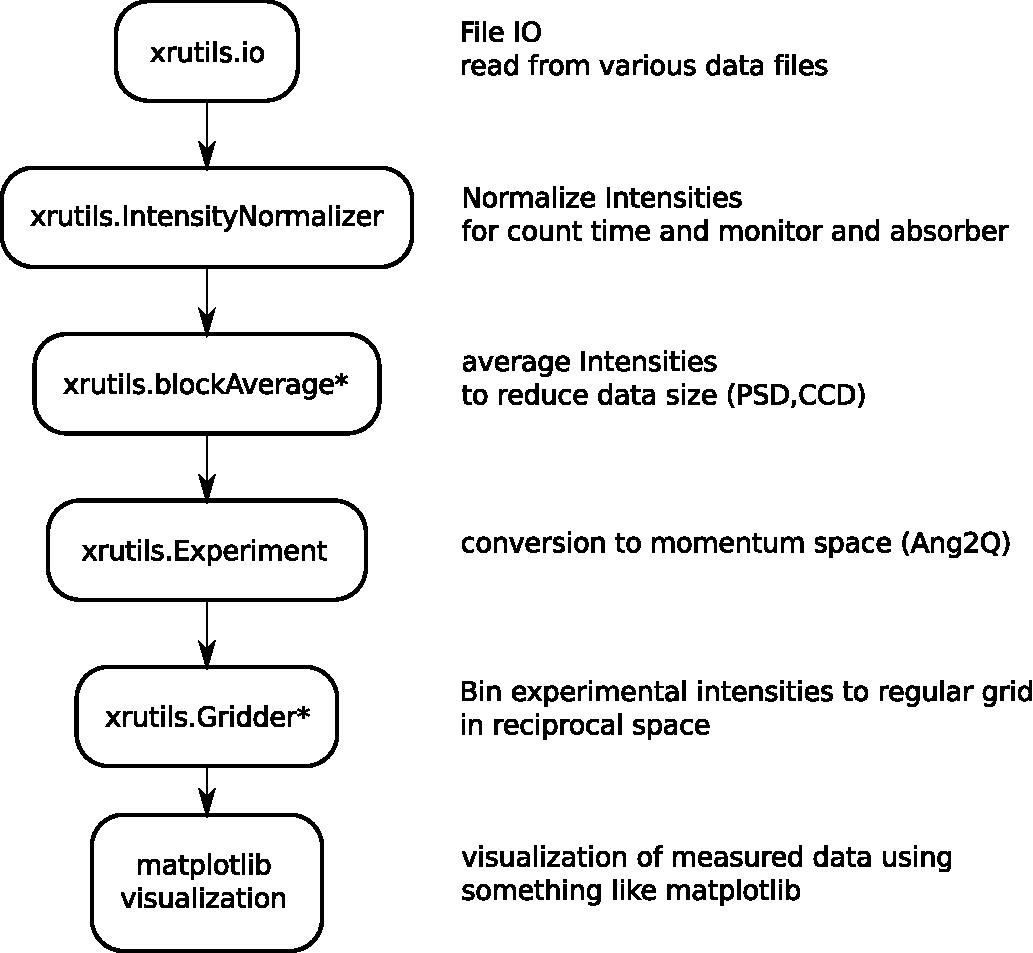
\includegraphics[width=0.8\linewidth]{pics/xrutils_usage}
 \caption{Flow diagram showing how to analyze x-ray diffraction data using {\tt xrutils}.}
 \label{fig:xrutils_usage}
\end{figure}

\section{Usage examples}

\subsection{spec-file from rotating anode}

The example shows the use of various parts of the xrutils package. It reads a \emph{spec}-file; saves the content into a HDF5 file; reads a particular scan and plots it as reciprocal space map.

\begin{lstlisting}[caption={reading a spec-file, saving it to HDF5, reading a particular scan, convert it to reciprocal space, plot it using matplotlib}]
import xrutils as xu
import numpy
import tables
import matplotlib.pyplot as plt

sample = "ko222"

cch = 501
chpdeg = 250.333
roi=[80,920]

#define substrate material + experimental class
InAs = xu.materials.InAs
expcub = xu.HXRD(InAs.Q(1,1,-2),InAs.Q(1,1,1))

#config psd and initialize a intensity normalizer
expcub.Ang2Q.init_linear('z+',cch,1024.,chpdeg=chpdeg,roi=roi)
RA_normalizer_psd = xu.IntensityNormalizer("MCA",time="Seconds",absfun=lambda d: d["PSDCORR"]/d["PSD"].astype(numpy.float))

# print theoretic angular positions
ang111 = expcub.Q2Ang(InAs.Q(1,1,1))
ang331 = expcub.Q2Ang(InAs.Q(3,3,1))
ang224 = expcub.Q2Ang(InAs.Q(2,2,4))
print " hkl\t%10s\t%10s\t%10s" %("om","tt","phi")
print "-------------------------------------------------------"
print " 111\t %10.3f\t%10.3f\t%10.3f" %(ang111[1],ang111[2],ang111[0])
print " 331\t %10.3f\t%10.3f\t%10.3f" %(ang331[1],ang331[2],ang331[0])
print " 224\t %10.3f\t%10.3f\t%10.3f" %(ang224[1],ang224[2],ang224[0])

#read spec file and save to HDF5
try: s
except NameError: s = xu.io.SPECFile(sample+".spec")
else: s.Update()

h5file = "./data/"+sample+".h5"
try: h5.isopen
except NameError:
    h5 = tables.openFile(h5file,mode='a')
else: 
    if not h5.isopen:
        h5 = tables.openFile(h5file,mode='a')
s.Save2HDF5(h5)

# read reciprocal space map from HDF5 file and plot it

uom = 12.7279 # aligned angular positions
utt = 25.4447
[thdel,thom,thtt] = expcub.Q2Ang(InAs.Q(1,1,1))

# parse map from file (omega scan around InAs(111) with PSD)
MAP = numpy.zeros(0)
for i in [17,]:
    exec ("scan = h5.root.%s.scan_%d.data.read()" %(sample,i))
    if MAP.dtype == numpy.float64:  MAP.dtype = scan.dtype
    MAP = numpy.append(MAP,scan)
                
# normalize intensity and apply region of interests
PSDRAW = RA_normalizer_psd(MAP)
PSD = xu.blockAveragePSD(PSDRAW, 1, roi=roi)
# conversion to reciprocal space
[qx,qy,qz] = expcub.Ang2Q.linear(MAP['Omega'],
                utt*numpy.ones(MAP['Omega'].size),
                delta=[ uom-thom, utt-thtt])

# grid intensity for visualization
gridder = xu.Gridder2D(200,200)
gridder(qy,qz,PSD)

# restrict dynamic range of measurement and make log10
ma = gridder.gdata.max()*10**(-0)
mi = gridder.gdata.max()*10**(-6)
INT = numpy.log10(numpy.minimum(
       numpy.maximum(gridder.gdata.transpose(),mi),ma))

# plot the map
plt.figure(); plt.clf()
cf = plt.contourf(gridder.xaxis, gridder.yaxis, INT,50)
plt.xlabel(r'$Q_y$ ($\AA$)'); plt.ylabel(r'$Q_z$ ($\AA$)')
#plt.subplots_adjust(bottom=0.12, top=0.92)
plt.colorbar(cf,ticks=numpy.arange(INT.min(),INT.max()+.1,
             round((INT.max()-INT.min())/10,1)),format="%.1f")
plt.figtext(0.76,0.93,r"$\log($Int$)$ (cps)") 
plt.savefig(sample+"_111rsm.png",dpi=200)

#close HDF5-datafile
h5.close()
\end{lstlisting}


\chapter[The materials submodule]{The {\tt materials} submodule}
% This file is part of xrayutilities.
%
% xrayutilities is free software; you can redistribute it and/or modify 
% it under the terms of the GNU General Public License as published by 
% the Free Software Foundation; either version 2 of the License, or 
% (at your option) any later version.
%
% This program is distributed in the hope that it will be useful,
% but WITHOUT ANY WARRANTY; without even the implied warranty of
% MERCHANTABILITY or FITNESS FOR A PARTICULAR PURPOSE.  See the
% GNU General Public License for more details.
%
% You should have received a copy of the GNU General Public License
% along with this program; if not, see <http://www.gnu.org/licenses/>.
%
% Copyright (C) 2009 Eugen Wintersberger <eugen.wintersberger@desy.de>
% Copyright (C) 2010 Dominik Kriegner <dominik.kriegner@gmail.com>

%%%documentation of the materials submodule

{\tt xrutils} provides a set of classes to describe crystal lattices and 
materials.

Examples show how to define a new material by definings its lattice and deriving a new material, furthermore materials can be used to calculate the structure factor of a Bragg reflection for an specific energy or the energy dependency of its structure factor for anomalous scattering.

\begin{lstlisting}[caption=defining a new material from scratch. This consists of an lattice with base and the type of atoms with elastic constantsof the material.]
import xrutils as xu

# defining a ZincBlendeLattice with two types of atoms and lattice constant a
def ZincBlendeLattice(aa,ab,a):
    #create lattice base
    lb = xu.materials.LatticeBase()
    lb.append(aa,[0,0,0])
    lb.append(aa,[0.5,0.5,0])
    lb.append(aa,[0.5,0,0.5])
    lb.append(aa,[0,0.5,0.5])
    lb.append(ab,[0.25,0.25,0.25])
    lb.append(ab,[0.75,0.75,0.25])
    lb.append(ab,[0.75,0.25,0.75])
    lb.append(ab,[0.25,0.75,0.75])
    
    #create lattice vectors
    a1 = [a,0,0]
    a2 = [0,a,0]
    a3 = [0,0,a]
    
    l = xu.materials.Lattice(a1,a2,a3,base=lb)    
    return l

# defining InP, no elastic properties are given, 
# helper functions exist to create the (6,6) elastic tensor for cubic materials 
InP  = xu.materials.Material("InP",ZincBlendeLattice(xu.elements.In, xu.elements.P,5.8687), numpy.zeros((6,6),dtype=numpy.double))
# InP is of course already included in the xu.materials module
\end{lstlisting}

\begin{lstlisting}[caption=calculation of the reflection strength of a Bragg reflection]
import xrutils as xu
import numpy

# defining material and experimental setup
InAs = xu.materials.InAs
energy= 8048 # eV

# calculate the structure factor for InAs (111) (222) (333)
hkllist = [[1,1,1],[2,2,2],[3,3,3]]
for hkl in hkllist:
    qvec = InAs.Q(hkl)
    F = InAs.lattice.StructureFactor(energy,qvec)
    print(" |F| = %8.3f" %numpy.abs(F))
\end{lstlisting}

\begin{lstlisting}[caption=energy dependency of the structure factor]
import xrutils as xu
import numpy
import matplotlib.pyplot as plt

# defining material and experimental setup
InAs = xu.materials.InAs
energy= numpy.linspace(500,20000,5000) # 500 - 20000 eV

F = InAs.lattice.StructureFactorForEnergy(energy,InAs.Q(1,1,1))

plt.figure(); plt.clf()
plt.plot(energy,F.real,'k-',label='Re(F)')
plt.plot(energy,F.imag,'r-',label='Imag(F)')
plt.xlabel("Energy (eV)"); plt.ylabel("F"); plt.legend()
\end{lstlisting}

It is also possible to calculate the structure factor of atoms which may be needed for input into XRD simulations.

\begin{lstlisting}[caption=components of the structure factor for simulations]
# f = f0(|Q|) + f1(en) + j * f2(en)
import xrutils as xu
import numpy

Fe = xu.materials.elements.Fe # iron atom
Q = numpy.array([0,0,1.9],dtype=numpy.double)
en = 10000 # energy in eV

print "Iron (Fe): E: %9.1f eV" % en
print "f0: %8.4g" % Fe.f0(numpy.linalg.norm(Q))
print "f1: %8.4g" % Fe.f1(en)
print "f2: %8.4g" % Fe.f2(en)
\end{lstlisting}




\chapter[The Experiment classes]{The {\tt Experiment} classes}
% This file is part of xrayutilities.
%
% xrayutilities is free software; you can redistribute it and/or modify
% it under the terms of the GNU General Public License as published by
% the Free Software Foundation; either version 2 of the License, or
% (at your option) any later version.
%
% This program is distributed in the hope that it will be useful,
% but WITHOUT ANY WARRANTY; without even the implied warranty of
% MERCHANTABILITY or FITNESS FOR A PARTICULAR PURPOSE.  See the
% GNU General Public License for more details.
%
% You should have received a copy of the GNU General Public License
% along with this program; if not, see <http://www.gnu.org/licenses/>.
%
% Copyright (C) 2010 Dominik Kriegner <dominik.kriegner@aol.at>

%%%documentation of the Experimental classes included in xrutils

The {\tt Experiment} class and derived classes provide routines to help performing X-ray diffraction experiments. This includes methods to calculate the diffraction angles needed to align samples and to convert data between angular and reciprocal space. The conversion from angular to reciprocal space is implemented very general. Users should in normal cases only need the initialized routines in the Experiment classes.

\section{Qconversion - general angular to momentum space conversion}

Conversion of angular coordinates to reciprocal space can be tedious if one needs specialized code for several machines. This is an attempt in which it is tried to provide a more general solution to the problem of the conversion. Therefore the code is not only feeded with the angular coordinates but also with a description of the used goniometer geometry. The conversion for scans with an point detector and also routines for PSD (linear) and CCD (area) detectors are implemented.

\section{mathematical background}

 For the routine to work for general goniometer setups a description of the goniometer type is needed. This is done in the following coordinate system:

\begin{figure}[H]
 \centering
 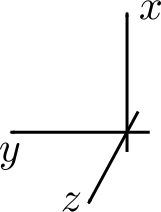
\includegraphics[width=0.13\linewidth]{pics/coordinate_system}
 \caption{Used right handed coordinate system: x .. up; y .. left; z .. towards the viewer}
 \label{fig:def_coordinate_system}
\end{figure}

\subsection*{description of the rotation axis}

In general always look from arrow head of the axis towards the tail, then
\begin{itemize}
 \item clockwise rotation means left-handed (negative),
 \item and anti-clockwise meand right-handed (positive)
\end{itemize}

i.\,e.: clockwise/left-handed rotation around the x-axis is decribed by the following rotation matrix:

\begin{align}
 R = \begin{pmatrix} 1 & 0 & 0 \\ 0 & \cos \alpha & \sin \alpha \\ 0 & -\sin\alpha & \cos \alpha \end{pmatrix}
\end{align}

The routines need to be supplied with the goniometer geometry. Therefore the goniometer axes are specified by their axis [xyz] and their sense of rotation [+-]. This description needs to be supplied for the sample and detector circles for the case where all axis are at zero position starting with the outermost circle.

For the Seifert XRD system this would mean:
Sample circles: Omega + Chi + Phi -> ["x+","y+","z+"]
Detector circles: Theta -> ["x+",]

\subsection{calculation of the momentum transfer}

The calculation the reciprocal space coordinates from angular positions is done as described in J. Appl. Cryst. (1999) {\bf 32} 614. Therefore we introduce the following nomenclatur:

\begin{nomenclatur}
 \item[\vec k_{i,f}] incidence and exiting wave vector of the x-ray radiation
 \item[\vec h_c] reciprocal space vector in carthesian coordinate system of the crystal
 \item[\vec h_u] reciprocal space vector in the coordinate system of the inner most circle of the goniometer
 \item[\vec h] reciprocal space vector in laboratory coordinate system
 \item[\vec Q_L] momentum transfer in laboratory coordinate system
 \item[\mat U] orientation matrix of the crystal
 \item[\mat S] rotation matrix for the sample goniometer
 \item[\mat D] rotation matrix for the detector circles
\end{nomenclatur}

To observe diffraction at position of $\vec h_c$ in reciprocal space the condition
\begin{align}
 \vec h = \vec Q_L
\label{eq:fundamental_law}
\end{align}
must be met. Where
\begin{align}
 \vec h = \mat R \vec h_u = \mat S \mat U \vec h_c
\end{align}
and
\begin{align}
 \vec Q_L = \vec k_f - \vec k_i = \left( \mat D - \mat 1 \right) \vec k_i
\end{align}

The reciprocal space position $\vec h_c$ can than be calculated from Eq.~\ref{eq:fundamental_law} as
\begin{align}
 \vec h_c = \left( \mat S \mat U \right)^{-1} \left(\mat D - \mat 1 \right) \vec k_i
 \label{eq:momentum_space_conversion}
\end{align}

The rotation matrices $\mat S$ and $\mat D$ can be deduces from the description of the goniometer by multipliing the rotation matrices from each circle starting with the outer most.

\begin{align}
 \mat D, \mat S = \text{(outer most)} \cdot \dots \cdot \text{(inner most)}
\end{align}

Note that all matrices are orthonormal, because they correspond to some basis transformation form one to another orthonormal coordinate system. Only the matrix $\mat B$ which describes the transformation from the Miller indices $\vec h$ to the reciprocal space vector $\vec h_c$ must not be orthonormal (e.\,g. hexagonal crystals).

\begin{align}
 \vec h_c = \mat B \vec h
\end{align}

\section{implementation}

The numerical expensive routines are coded in C because they seem to be a performance critical step in the analysis of XRD data. Because of the general form of the code some overhead must be excepted. Some wrapper functions are written in Python because of the ability of the fast coding.

\subsection*{general things}

\begin{itemize}
 \item all matrices are stored row-major (C standard) in linear array
 \item angles are passed as radians
\end{itemize}

\subsection*{rotation matrices}

The used rotation matrices follow the rotation sense definition given earlier. In the following the rotation matrices for the positive rotation around the coordinate axes are given.

\begin{align}
\mat {R_x} ( \alpha ) = \begin{pmatrix}
                       1 & 0 & 0 \\
               0 & \cos\alpha & -\sin\alpha \\
               0 & \sin\alpha & \cos\alpha
                      \end{pmatrix}
\end{align}

\begin{align}
\mat {R_y} ( \alpha ) = \begin{pmatrix}
                       \cos\alpha & 0 & \sin\alpha \\
               0 & 1 & 0 \\
               -\sin\alpha & 0 & \cos\alpha
                      \end{pmatrix}
\end{align}

\begin{align}
\mat {R_z} ( \alpha ) = \begin{pmatrix}
               \cos\alpha & -\sin\alpha & 0 \\
               \sin\alpha & \cos\alpha  & 0 \\
               0 & 0 & 1
                      \end{pmatrix}
\end{align}

For the

\subsection*{matrix inversion}
The needed matrix inversion of a $3\times3$ matrix $\mat A$ is done using the adjugate matrix formula

\begin{align}
 \mat A^{-1} = \frac{\operatorname{adj} \mat A} {\operatorname{det} \mat A} \text{ ,}
\end{align}
which yields the formula
\begin{align}
 \mat A^{-1} = \begin{pmatrix} a_{00} & a_{01} & a_{02} \\
                               a_{10} & a_{11} & a_{12} \\
                               a_{20} & a_{21} & a_{22} \end{pmatrix}
= \frac{1}{\operatorname{det}\mat A}
\begin{pmatrix}
a_{11} a_{22} - a_{12} a_{21} & a_{02} a_{21} - a_{01} a_{22} & a_{01} a_{12} - a_{02} a_{11} \\
a_{12} a_{20} - a_{10} a_{22} & a_{00} a_{22} - a_{02} a_{20} & a_{02} a_{10} - a_{00} a_{12} \\
a_{10} a_{21} - a_{11} a_{20} & a_{01} a_{20} - a_{00} a_{21} & a_{00} a_{11} - a_{01} a_{10}
\end{pmatrix}
\end{align}
with
\begin{align}
 \operatorname{det} \mat A = a_{00}a_{11}a_{22} + a_{01}a_{12}a_{20} + a_{02}a_{10}a_{21} - a_{02}a_{11}a_{20} - a_{01}a_{10}a_{22} - a_{00}a_{12}a_{21} \text{ .}
\end{align}

\section{1D and 2D detectors}

The C-code for linear and area detectors performs an exact conversion from real to momentum space by assuming the knowledge of the position and orientation of the detector in real space as well as its pixel distance. If the position and pixel size is not known it can be calculated from the channels per degree ($N$) which are mostly determined while recording measurements.

Therefore a distance of $d=1$ (units are irrelevant here) is assumed and the corresponding pixel size is calclulated via

\begin{align}
 w_\text{Pixel} = \frac{2d}{N} \tan\unit{0.5}{\degree}
\end{align}

The channels per degree of the detector are mostly determined symmetric with respect to the center channel. Therefore a factor $2$ and angle \unit{0.5}{\degree} was introduced (see Fig.~\ref{fig:detector_chpdeg}).

\begin{figure}[H]
 \centering
 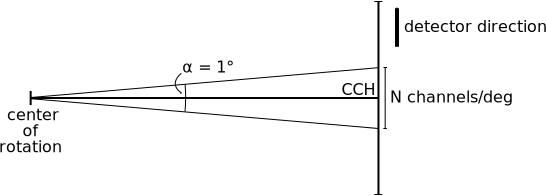
\includegraphics[width=0.6\linewidth]{pics/linear_detector_chpdeg}
 \caption{Illustration of a linear detector and channels per degree. (CCH: \underline{c}enter \underline{ch}annel)}
 \label{fig:detector_chpdeg}
\end{figure}

For the conversion to momentum space not only the distance $d$, pixel width $w$ but also the detector direction is needed (Fig.~\ref{fig:detector_chpdeg}). The coordinate system is assumed to be the one defined in Fig.~\ref{fig:def_coordinate_system}.

The conversion is then done similar to Eq.~\ref{eq:momentum_space_conversion}. For the calculation of $\vec k_f$ the direction vector of each detector pixel $\vec{\hat r}_d$ must be used in the conversion routine, which leads to the following formulation:

\begin{align}
\vec h_c = \left( \mat S \mat U \right)^{-1} \left(|\vec k_i| \mat D \vec{\hat r}_d - \vec k_i  \right)
 \label{eq:momentum_space_conversion_detector}
\end{align}


\section{HXRD experiments}

Methods for high angle x-ray diffraction experiments. Mostly for experiments performed in coplanar scattering geometry. An example will be given for the calculation of the position of Bragg reflections.

\begin{lstlisting}[caption=calculation of angles for Si Bragg reflections]
import xrutils as xu

Si = xu.materials.Si  # load material from materials submodule

# initialize experimental class with directions from experiment
exp = xu.HXRD(Si.Q(1,1,-2),Si.Q(1,1,1))

# calculate angles and print them to the screen
angs = exp.Q2Ang(Si.Q(1,1,1))
print "Si (111)"
print "om: %8.3f" %angs[1]
print "tt: %8.3f" %angs[2]

angs = exp.Q2Ang(Si.Q(2,2,4))
print "Si (224)"
print "om: %8.3f" %angs[1]
print "tt: %8.3f" %angs[2]
\end{lstlisting}


\section{GID experiments}

Implementation of this class is missing

\section{Powder diffraction}

The powder diffraction class is able to convert powder scans from angular to reciprocal space and furthermore powder scans of materials can be simulated in a very easy way.

\begin{lstlisting}[caption=conversion between angular and reciprocal space using the powder diffraction class]
import xrutils as xu

energy = 10000 # eV
powder = xu.Powder(xu.materials.Si,en=energy) # just give some material

# convert absolute q-space value to theta = 2theta/2
theta = powder.Q2Ang(2.0) # 2.0 A^{-1}
# and back
qpos = powder.Ang2Q(theta) # qpos = 2.0
\end{lstlisting}

\begin{lstlisting}[caption=simulation of an powder diffraction scan and two distinct ways of plotting the results]
import xrutils as xu
import matplotlib.pyplot as plt

energy = (2*8048 + 8028)/3. # copper k alpha 1,2

# creating Indium powder
In_powder = xu.Powder(xu.materials.Indium,en=energy)
# calculating the reflection strength for the powder
In_powder.PowderIntensity()

# convoluting the peaks with a gaussian in q-space
peak_width = 0.01 # in q-space
resolution = 0.0005 # resolution in q-space
In_th,In_int = In_powder.Convolute(resolution,peak_width)

plt.figure(); plt.clf()
ax1 = plt.subplot(111)
plt.xlabel(r"2Theta (deg)"); plt.ylabel(r"Intensity")
# plot the convoluted signal
plt.plot(In_th*2,In_int/In_int.max(),'k-',label="Indium powder convolution")
# plot each peak in a bar plot
plt.bar(In_powder.ang*2, In_powder.data/In_powder.data.max(), width=0.3, bottom=0, linewidth=0, color='r',align='center', orientation='vertical',label="Indium powder bar plot")

plt.legend(); ax1.set_xlim(15,100); plt.grid()
\end{lstlisting}


\chapter[The io submodule]{The {\tt io} submodule}
% This file is part of xrayutilities.
%
% xrayutilities is free software; you can redistribute it and/or modify 
% it under the terms of the GNU General Public License as published by 
% the Free Software Foundation; either version 2 of the License, or 
% (at your option) any later version.
%
% This program is distributed in the hope that it will be useful,
% but WITHOUT ANY WARRANTY; without even the implied warranty of
% MERCHANTABILITY or FITNESS FOR A PARTICULAR PURPOSE.  See the
% GNU General Public License for more details.
%
% You should have received a copy of the GNU General Public License
% along with this program; if not, see <http://www.gnu.org/licenses/>.
%
% Copyright (C) 2009 Eugen Wintersberger <eugen.wintersberger@desy.de>
% Copyright (C) 2010 Dominik Kriegner <dominik.kriegner@aol.at>

%%%documentation of the io submodule

The {\tt io} submodule provides classes for reading x-ray diffraction data in
various formats. 

\section{Reading SPEC files}

Working with spec files in xrutils can be done in two distinct ways. 
\begin{enumerate}
 \item parsing the spec file for scan headers; and parsing the data only when needed
 \item parsing the spec file for scan headers; parsing all data and dump them to an HDF5 file; reading the data from the HDF5 file. 
\end{enumerate}
Both methods have their pros and cons. For example when you parse the spec-files over a network connection you need to re-read the data again over the network if using method 1) whereas you can dump them to a local file with method 2). But you will parse data of the complete file while dumping it to the HDF5 file. 

Both methods work incremental, so they do not start at the beginning of the file when you reparse it, but start from the last position they were reading.

An working example for methode two is given in the following.

\begin{lstlisting}[caption=parsing a SPEC file and read data (1) or dumping the data to an HDF5 file (2)]
import tables
import xrutils as xu

# open spec file or use open SPECfile instance
try: s
except NameError:
    s = xu.io.SPECFile("sample_name.spec",path="./specdir")

# method (1)
scan10 = s[9] # Returns a SPECScan class
scan10.ReadData()
scan10data = scan10.data

# method (2)
h5file = "./h5dir/h5file.h5"
try: h5.isopen # open HDF5 file or use open one
except NameError:
    h5 = tables.openFile(h5file,mode='a')
else:
    if not h5.isopen: h5 = tables.openFile(h5file,mode='a')
s.Save2HDF5(h5) # save content of SPEC file to HDF5 file
# read data from HDF5 file
scan10data = h5.root.sample_name.scan_10.data.read()
\end{lstlisting}

\begin{lstlisting}[caption=reparse the SPEC file for new scans and reread the scans (1) or update the HDF5 file(2)]
...

s.Update() # reparse for new scans in open SPECFile instance

# reread data method (1)
scan10 = s[9] # Returns a SPECScan class
scan10.ReadData()
scan10data = scan10.data 

# reread data method (2)
s.Save2HDF5(h5) # save content of SPEC file to HDF5 file
# read data from HDF5 file
scan10data = h5.root.sample_name.scan_10.data.read()
\end{lstlisting}

\section{Reading EDF files}

EDF files are mostly used to store CCD frames at ESRF. This format is therefore used in combination with SPEC files. In an example the EDFFile class is used to parse the data from EDF files and store them to an HDF5 file. HDF5 if perfectly suited because it can handle large amount of data and compression.

\begin{lstlisting}[caption=script to parse and plot a reciprocal space map recorded with Seifert's XRD control software]
import tables 
import xrutils as xu
import numpy

specfile = "specdir/mo3211b.dat"
h5file = "h5dir/mo3211b.h5"
h5 = tables.openFile(h5file,mode='a')

s = xu.io.SPECFile(specfile,path=specdir)
s.Save2HDF5(h5) # save to hdf5 file

# read ccd frames from EDF files
for i in range(1,1000,1):
    efile = "edfdir/sample_%04d.edf" %i
    e = xu.io.edf.EDFFile(efile,path=specdir)
    e.ReadData()
    g5 = h5.createGroup(h5.root,"frelon_%04d" %i)
    e.Save2HDF5(h5,group=g5)

h5.close()
\end{lstlisting}

\section{Reading Bruker CCD data}

\section{Reading Radicon files}

Usage of Radicon files is deprecated. They were used by an old control software of Radicon. There are functions to read this format!

\section{Reading Seifert ASCII files}

Two functions to read ASCII data from Seifert's XRD control software are available. One which reads single scans most times recorded with the point detector and the other one for parsing files which contain multiple scans (e.g.: RSMs recorded with the PSD).

\begin{lstlisting}[caption=script to parse and plot a reciprocal space map recorded with Seifert's XRD control software]
import xrutils as xu
import matplotlib.pyplot as plt
import numpy

exp111 = xu.HXRD([1,1,-2],[1,1,1])
# 
data = xu.io.SeifertMultiScan('seifertmultiscan.nja','T','O')

om  = data.m2_pos[:,numpy.newaxis]*numpy.ones(data.int.shape)
tt  = data.sm_pos[numpy.newaxis,:]*numpy.ones(data.int.shape)

[qdummy,qy,qz] = exp111.Ang2Q(om,tt,0.)

gridder = xu.Gridder2D(300,300)
gridder(qy,qz,data.int)
INT = numpy.log10(gridder.gdata.transpose().clip(0.01,1e9))

plt.figure(); plt.clf()
plt.contourf(gridder.xaxis,gridder.yaxis,INT,50)
plt.xlabel(r'Qx'); plt.ylabel(r'Qz'); plt.colorbar()
\end{lstlisting}

\begin{lstlisting}[caption=script to parse and plot a single scan recorded with Seifert's XRD control software]
import xrutils as xu
import matplotlib.pyplot as plt

data = xu.io.SeifertScan('seifert.nja')

plt.figure(); plt.clf()
plt.plot(d.data[:,0],d.data[:,1],'k-')
plt.xlabel(r'scan axis (deg)'); plt.ylabel(r'Int (cps)'); plt.grid()
\end{lstlisting}


%\chapter[The vis submodule]{The {\tt vis} submodule}
%% This file is part of xrayutilities.
%
% xrutils is free software; you can redistribute it and/or modify 
% it under the terms of the GNU General Public License as published by 
% the Free Software Foundation; either version 2 of the License, or 
% (at your option) any later version.
%
% This program is distributed in the hope that it will be useful,
% but WITHOUT ANY WARRANTY; without even the implied warranty of
% MERCHANTABILITY or FITNESS FOR A PARTICULAR PURPOSE.  See the
% GNU General Public License for more details.
%
% You should have received a copy of the GNU General Public License
% along with this program; if not, see <http://www.gnu.org/licenses/>.
%
% Copyright (C) 2009 Eugen Wintersberger <eugen.wintersberger@desy.de>

%%%documentatino of the visualizatino submodule vis



\end{document}
